\documentclass[10pt,twocolumn,letterpaper]{article}

% Official CVPR author kit (cvpr-org/author-kit, package dated 2027).
% Final mode: this is a course report, not a blind review copy.
\usepackage[pagenumbers]{cvpr}
\usepackage[pagebackref,breaklinks,colorlinks]{hyperref}
% XeTeX (Tectonic) has no Unicode shapes for the Type~1 times package
% that cvpr.sty loads. Nimbus Roman is the Times-compatible face that
% package selects. The four files live in report/fonts with their license.
\usepackage{fontspec}
\setmainfont{NimbusRoman}[
  Path=fonts/,
  Extension=.otf,
  UprightFont=*-Regular,
  BoldFont=*-Bold,
  ItalicFont=*-Italic,
  BoldItalicFont=*-BoldItalic
]

\def\confName{CVPR}
\def\confYear{2026}

\title{MLPs, CNNs, Autoencoders, SVMs and Clustering on CIFAR-10}

\author{Praveen\\
Roll m26csa003\\
Repository: not yet published\\
Commit: none yet (this directory is not a git repository)}

\begin{document}
\maketitle

\begin{abstract}
We study why a multilayer perceptron is weak on CIFAR-10, whether a convolutional bottleneck stores class information, and how a frozen convolutional code behaves under a kernel SVM and under clustering. One stratified split, seed 26003, holds out 5{,}000 of the 50{,}000 official training images for every choice. The official test set is scored only after those choices. A matched CNN reaches $73.9\%{\pm}3.0$ test accuracy against $50.4\%{\pm}0.2$ for a matched MLP. A wider MLP and stronger regularisation do not close the gap. A fixed spatial permutation removes the CNN's lead. Three autoencoders, differing only in bottleneck width, are selected by validation MSE, and a denoiser improves pixels without restoring the classifier. A polynomial SVM on frozen CNN features, selected on validation, scores $72.35\%$ on the test set; $k$-means on the same features does not.
\end{abstract}

\noindent\textbf{Submission record.}
Name: Praveen.
Roll: m26csa003.
GitHub repository: not yet published.
Final commit hash: none. The project directory is not a git repository, so no hash is available to report.

\section{Introduction}
CIFAR-10 is small, varied in pose and background, and balanced across ten classes~\cite{krizhevsky2009cifar}. A dense layer ties each weight to one pixel position, so a local pattern that moves must be relearned. A convolution reuses one filter at every position. This report tests that explanation against capacity and overfitting, then asks whether the same spatial bias is what a CNN is using, whether an autoencoder's code keeps class identity, and whether a kernel classifier and a label-free clustering of one frozen code agree.

Every comparison that selects a model, a learning rate, a bottleneck, a kernel, or a number of clusters is written down before the corresponding run and is decided on the validation split. Reused models are named with the question that introduced them.

\section{Dataset and protocol}
The official CIFAR-10 training pool has 50{,}000 images and the test set has 10{,}000, with 5{,}000 and 1{,}000 images in each class~\cite{krizhevsky2009cifar}. Seed 26003, the digits of roll m26csa003 in order, draws one stratified split of the training pool: 4{,}500 train and 500 validation images in every class. The indices are stored in \texttt{splits/split\_seed26003.npz}. Train and validation do not overlap and together they are the official training set. A second draw from the same seed matches the file; the loader refuses to replace it.

Pixels are scaled to $[0,1]$. Classifiers subtract the training-split per-channel mean and divide by the population standard deviation, both reduced in float64. The saved means are $0.4914$, $0.4821$, $0.4466$ and the standard deviations are $0.2469$, $0.2434$, $0.2615$. Validation and test pixels are not included. Autoencoders stay in $[0,1]$, so mean squared error is on the pixel scale. PSNR uses a peak of 1.

Training uses PyTorch~2.1.2 with CUDA~11.8 and torchvision~0.16.2~\cite{paszke2019pytorch}. The SVM and the clustering use scikit-learn~1.3.2~\cite{pedregosa2011sklearn}. Classifier and autoencoder runs that produced the tables ran on an NVIDIA A30. The optimiser is AdamW~\cite{kingma2015adam,loshchilov2019adamw} with betas $(0.9, 0.999)$ and a cosine schedule to zero. Seeds fix Python, NumPy and PyTorch. cuDNN is set deterministic; atomic adds can still differ, so Question~1 and Question~2 report three seeds (26003, 26004, 26005) as a mean and a sample standard deviation. The checkpoint is the earliest epoch with the best validation score. Sample standard deviation uses divisor $n-1$.

\section{Question 1: MLP versus CNN}
\subsection{Comparison}
The reason under test is missing spatial weight sharing. Two alternatives are locked in \texttt{configs/q1\_fairness.json} before training. A wide MLP asks whether the matched MLP is weak only because a matched budget forces it to be narrow. The same narrow MLP with dropout $0.3$ and weight decay $10^{-3}$ asks whether the problem is overfitting. No model is augmented and none uses batch normalisation.

The matched MLP is Linear $3072{\to}64$, ReLU, Linear $64{\to}64$, ReLU, Linear $64{\to}10$: 201{,}482 parameters. The matched CNN is three $3{\times}3$ convolutions with 64, 96 and 160 channels, ReLU and $2{\times}2$ max-pooling after each, then global average pooling and a linear head: 197{,}194 parameters, $2.1\%$ under the MLP. The wide MLP uses widths 512 and 256: 1{,}707{,}274 parameters. Weight decay is $10^{-4}$ except on the regularised MLP.

One learning rate is shared. An 8-epoch probe on the matched MLP and the matched CNN scores each candidate by the mean of the two best validation accuracies. The scores are $0.5341$ at $3{\times}10^{-4}$, $0.6022$ at $10^{-3}$, and $0.6263$ at $3{\times}10^{-3}$. The rule selects $3{\times}10^{-3}$. The MLP's own probe scores at $10^{-3}$ and $3{\times}10^{-3}$ are $0.5316$ and $0.5304$, so the shared rate is not an obvious handicap for the MLP. Final training is 30 epochs, batch 128. The wide and regularised MLPs do not get a private search.

\subsection{Test results}
Table~\ref{tab:q1} is the official test accuracy after validation selection. The CNN leads by about 23 points. About $8.5$ times as many parameters add about two points. Dropout and a stronger weight decay do not raise test accuracy. The wide MLP's training accuracy at the selected checkpoint is high and its test loss is high, so the extra weights overfit rather than close the architectural gap. The weakest CNN seed remains well above every MLP seed. Figure~\ref{fig:q1test} is the same table.

\begin{table}[t]
\centering
\caption{Question 1a. Mean $\pm$ sample standard deviation over three seeds. Test accuracy is the official test set.}
\label{tab:q1}
\small
\begin{tabular}{lrr}
\toprule
Model & Val. & Test \\
\midrule
Matched MLP & $.515{\pm}.003$ & $.504{\pm}.002$ \\
Matched CNN & $.742{\pm}.031$ & $.739{\pm}.030$ \\
Wide MLP & $.533{\pm}.005$ & $.527{\pm}.003$ \\
Regularised MLP & $.514{\pm}.003$ & $.505{\pm}.004$ \\
\bottomrule
\end{tabular}
\end{table}

\begin{figure}[t]
\centering
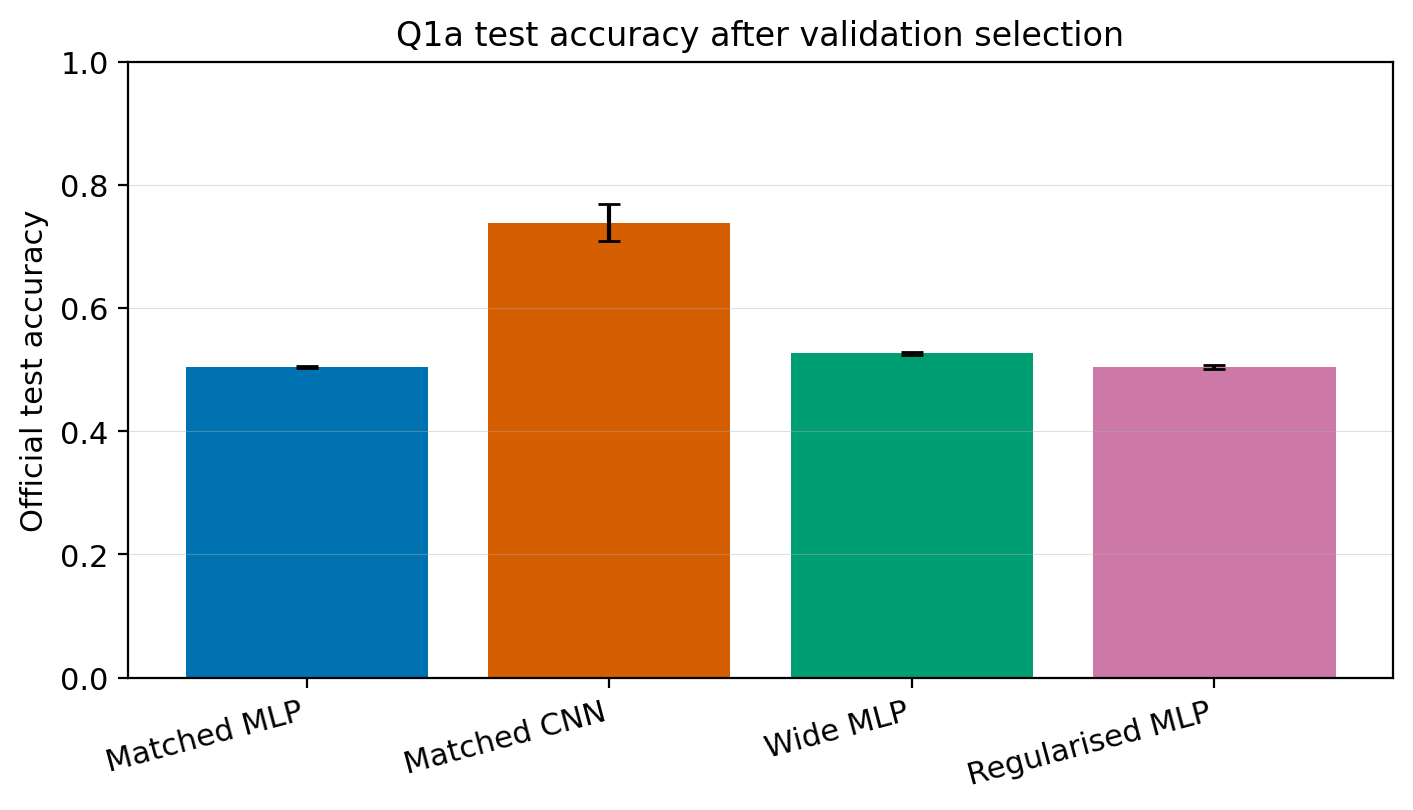
\includegraphics[width=\linewidth]{figures/q1_test.png}
\caption{Question 1a test accuracy. The bar is the three-seed mean and the whisker is the sample standard deviation.}
\label{fig:q1test}
\end{figure}

\subsection{Memorisation}
The wide MLP is trained again for 40 epochs with weight decay 0, which the plan excludes from the fair table, so that weight decay does not fight arbitrary labels~\cite{zhang2017understanding}. A stratified fraction of training labels is replaced by a uniform draw from the other nine classes. Validation labels stay clean. Every epoch records accuracy on the untouched training rows, fit to the random labels, accuracy on the true class of the corrupted rows, and clean validation accuracy.

The plan allows the claim ``useful structure before memorisation'' only if, at 20\% or 50\% noise, validation rises while the random-label fit is still near chance ($0.10$), and that fit keeps rising after validation has peaked. At 20\% noise, validation goes from $0.393$ to $0.458$ in five epochs while the noise fit stays at $0.070$--$0.081$. The peak is $0.463$ at epoch 19, when the noise fit is already $0.228$, and the noise fit then continues to $0.395$ as validation slips to $0.439$. At 50\% noise the peak is $0.318$ at epoch 6 with noise fit $0.090$; by epoch 40 the noise fit is $0.285$ and validation is $0.282$. The condition holds. The useful gain at 50\% is about two points. At 100\% noise the training loss stays at $\ln 10$ and both validation and the noise fit stay at chance, so this budget did not fit a fully random training set. Figure~\ref{fig:q1b} shows the four fractions.

\begin{figure*}[t]
\centering
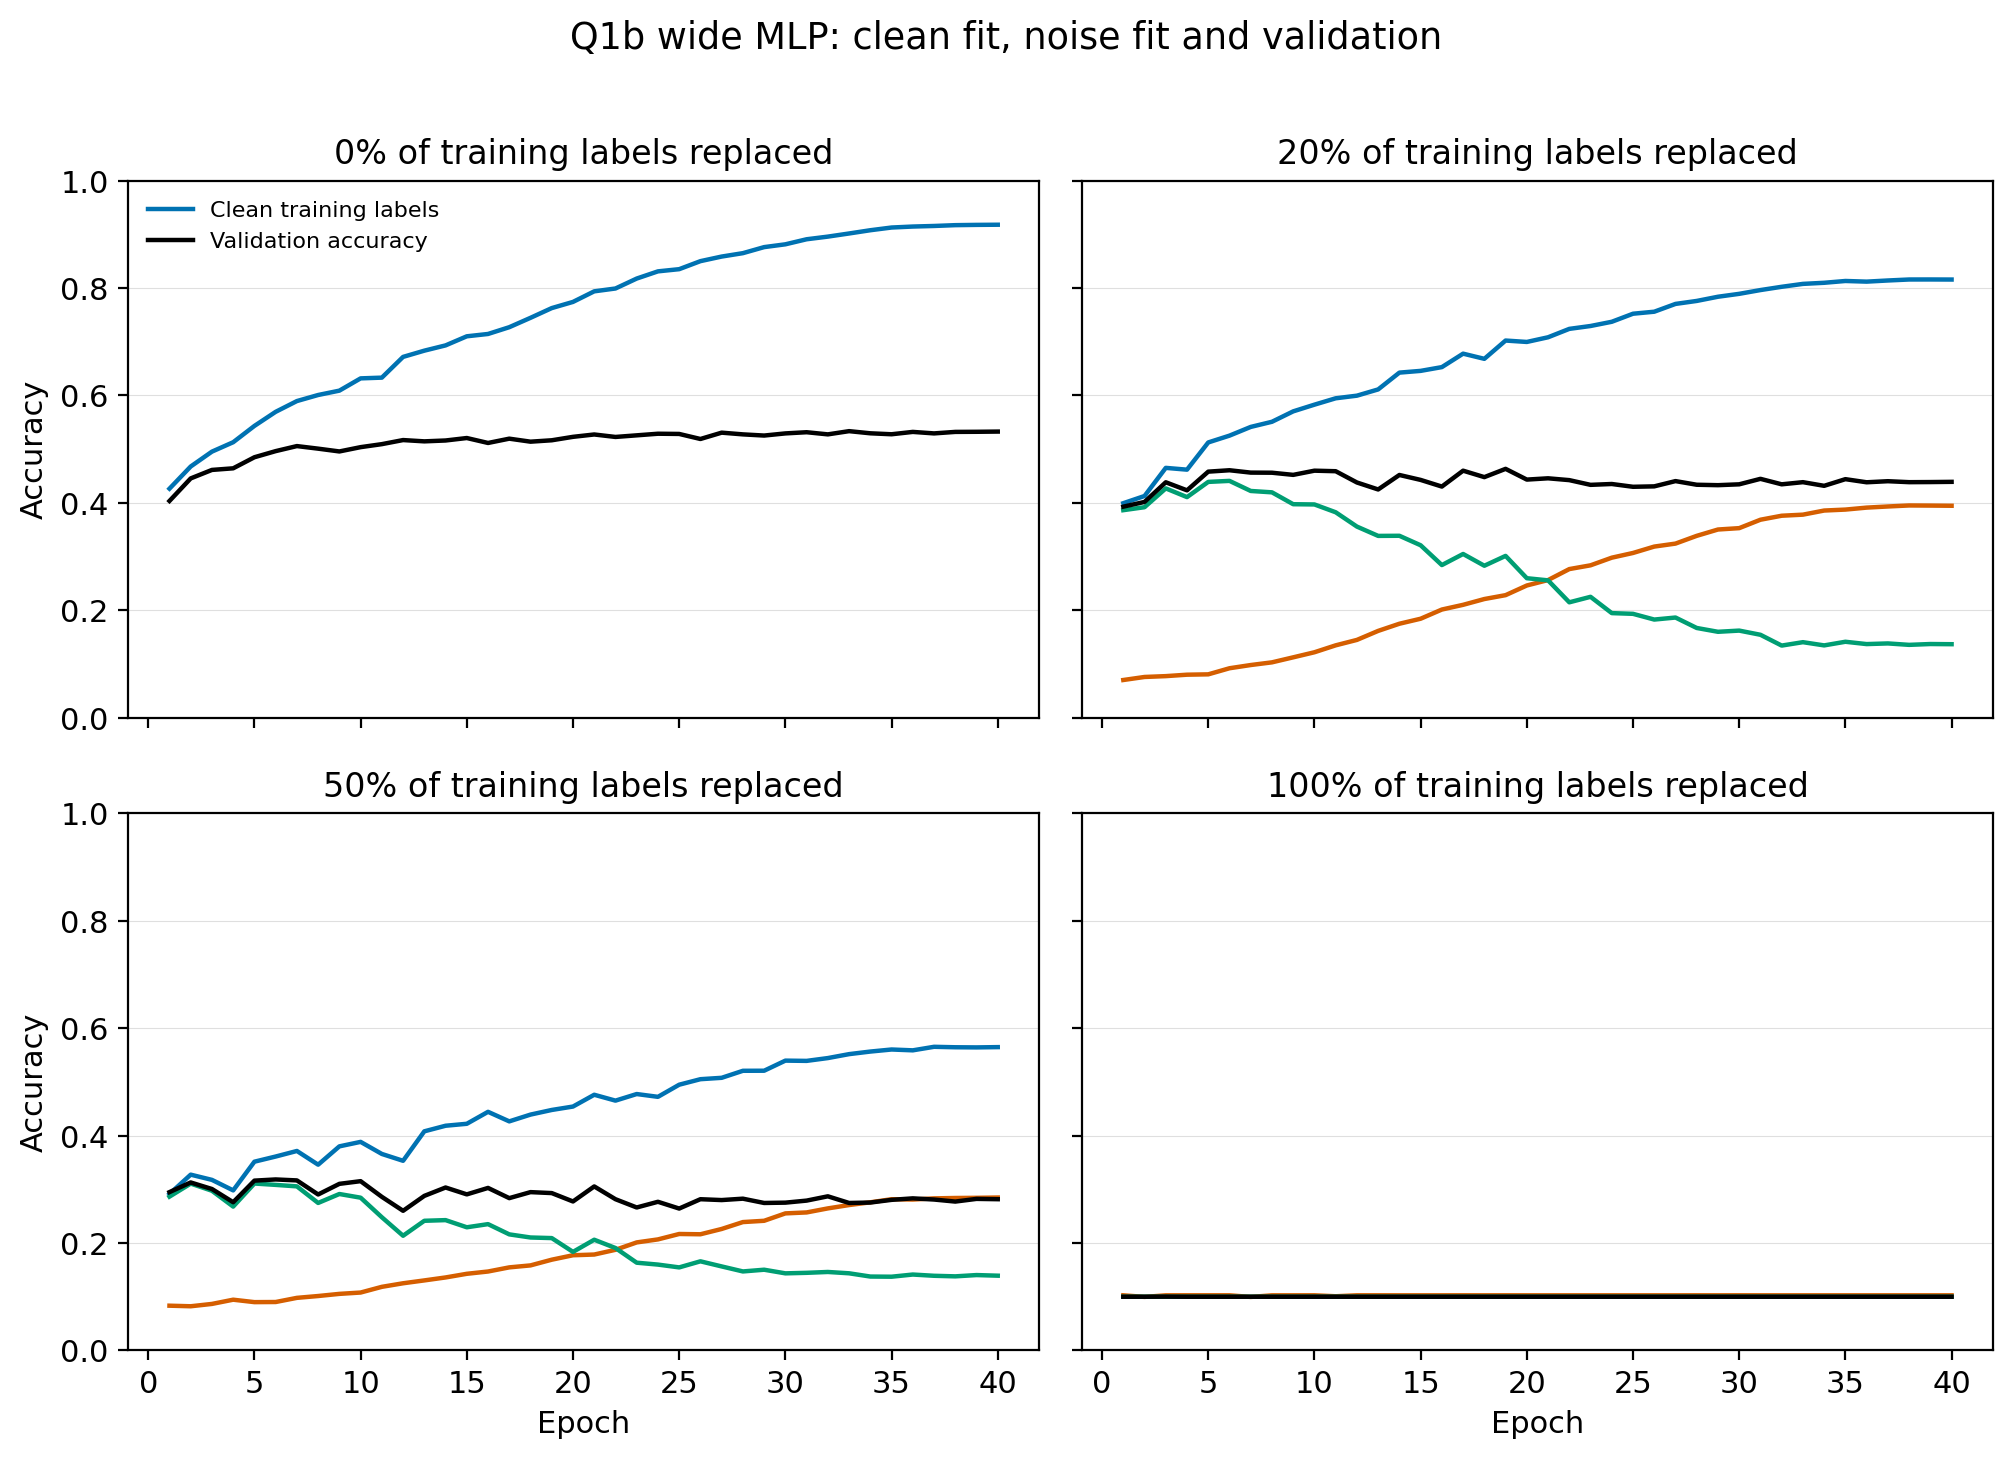
\includegraphics[width=0.92\textwidth]{figures/q1b.png}
\caption{Question 1b. Clean-label accuracy on the training rows that were not corrupted, fit to the random labels, accuracy on the true class of corrupted rows, and clean validation accuracy.}
\label{fig:q1b}
\end{figure*}

\section{Question 2: spatial structure and colour}
Part (a) does not train a new pair. It reuses the matched MLP and matched CNN from Question 1a, including their test numbers, which were recomputed from the same checkpoints and match Table~\ref{tab:q1}. Parts (b) and (c) retrain both architectures with the Question 1 recipe: learning rate $3{\times}10^{-3}$, weight decay $10^{-4}$, 30 epochs, three seeds, no new search.

Part (b) applies one permutation of the 1{,}024 spatial positions, drawn with \texttt{Generator(26003)} and saved, to every image and every channel. Pixel values inside a channel are reordered, not replaced, so the Question 1 channel statistics remain valid. The plan expected the MLP to stay within about three points of $0.504$ and the CNN to drop by much more than ten points. Part (c) replaces RGB by luma $0.2989R+0.5870G+0.1140B$, repeated on three channels so the parameter counts do not change. Grayscale mean and standard deviation are computed on the training split only. The plan treats a CNN that stays more than ten points above the MLP, and above $0.60$, as evidence for shape rather than colour.

\begin{table}[t]
\centering
\caption{Question 2 test accuracy, mean $\pm$ sample standard deviation over three seeds. Architectures were introduced in Question 1a.}
\label{tab:q2}
\small
\begin{tabular}{llr}
\toprule
Model & Condition & Test \\
\midrule
MLP & Clean & $.504{\pm}.002$ \\
MLP & Permuted & $.501{\pm}.003$ \\
MLP & Grayscale & $.419{\pm}.005$ \\
CNN & Clean & $.739{\pm}.030$ \\
CNN & Permuted & $.486{\pm}.028$ \\
CNN & Grayscale & $.612{\pm}.122$ \\
\bottomrule
\end{tabular}
\end{table}

\begin{figure}[t]
\centering
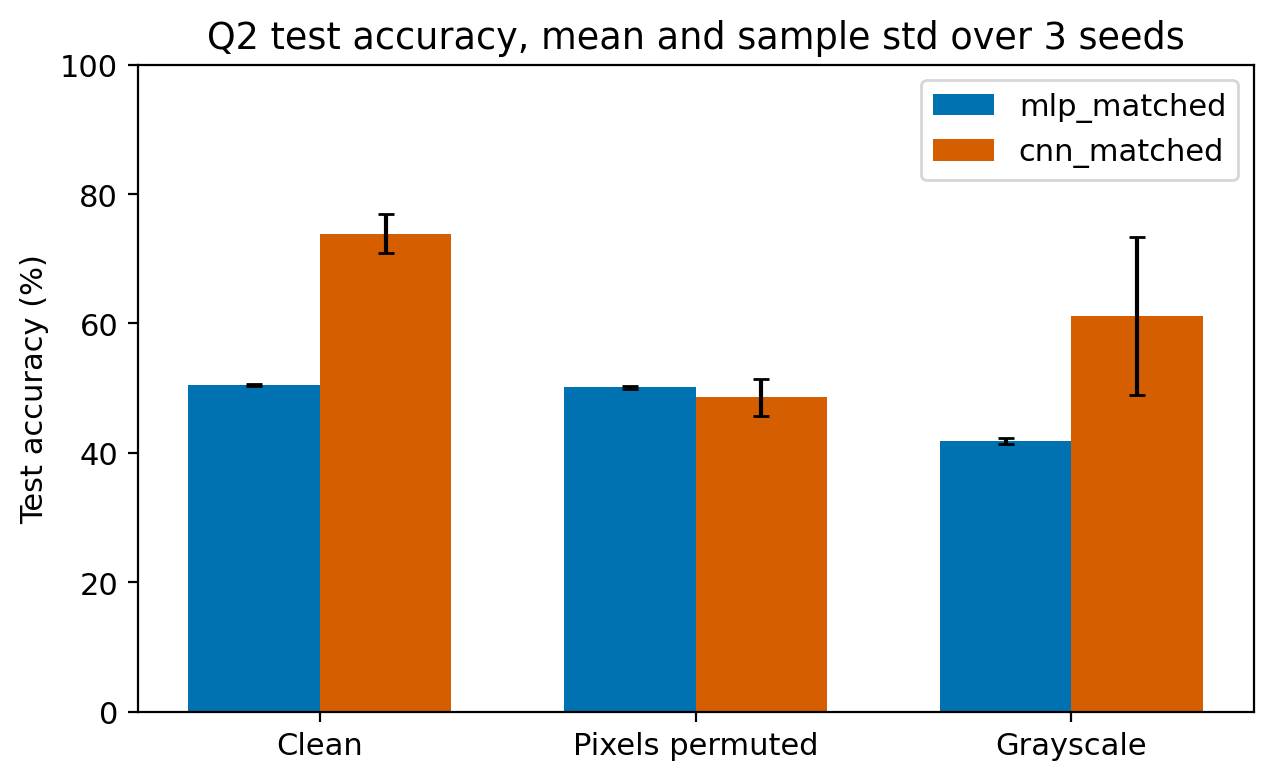
\includegraphics[width=\linewidth]{figures/q2_test.png}
\caption{Question 2 test accuracy under the three conditions.}
\label{fig:q2}
\end{figure}

Table~\ref{tab:q2} and Figure~\ref{fig:q2} match the plan for the permutation: the MLP stays at $0.501$ and the CNN falls from $0.739$ to $0.486$. On grayscale the mean gap remains, but the CNN seeds are $0.715$, $0.645$ and $0.476$. Seed 26005 has validation accuracy $0.490$. The ``above $0.60$'' sentence is therefore not true of every seed. Colour lowers both models. It does not, on the two stable seeds, explain the clean-image gap.

Confidence is the maximum softmax probability. For the matched CNN, mean confidence on correct versus incorrect test predictions is $0.862$ versus $0.648$ on clean images, $0.599$ versus $0.440$ after the permutation, and $0.717$ versus $0.515$ on grayscale (Figure~\ref{fig:q2c}). The fraction of errors with confidence at least $0.9$ falls from $0.148$ on clean images to $0.008$ after the permutation. The CNN becomes less sure when neighbourhoods are destroyed; it does not become confidently wrong.

\begin{figure}[t]
\centering
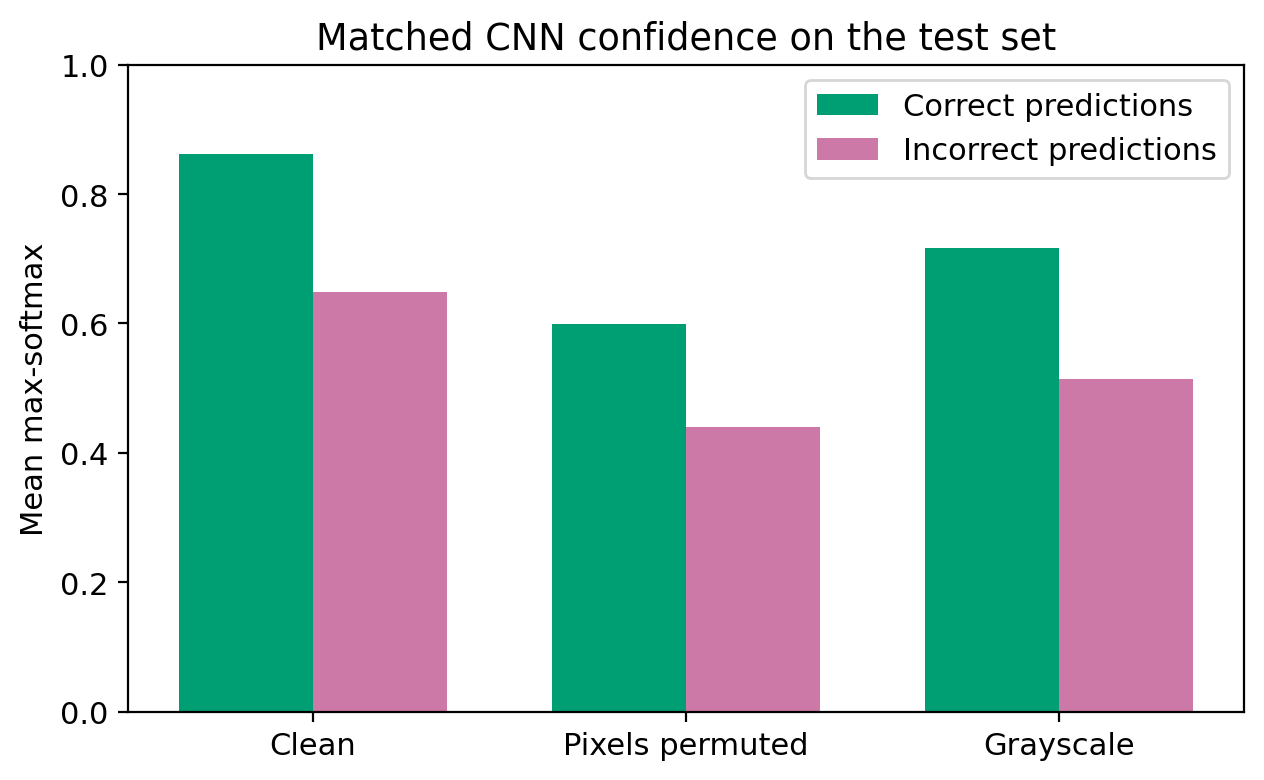
\includegraphics[width=\linewidth]{figures/q2_confidence.png}
\caption{Matched CNN mean max-softmax on correct and incorrect test predictions.}
\label{fig:q2c}
\end{figure}

\section{Question 3: autoencoders}
\subsection{Bottleneck}
Three convolutional autoencoders differ only in the width of the code: 32, 128 and 512 parameters of the two linear maps that enter and leave it. The encoder is three $3{\times}3$ convolutions (32, 64, 128 channels) with ReLU and $2{\times}2$ max-pooling. The code has no activation. The decoder maps the code back to $128{\times}4{\times}4$ and applies three stride-2 transposed convolutions and a sigmoid. Parameter counts are 267{,}843, 661{,}155 and 2{,}234{,}403. There is no batch normalisation. The loss is the mean squared error over the pixels of the batch,
\begin{equation}
\mathrm{MSE} = \frac{1}{BCHW}\sum_{b,c,h,w}\bigl(x_{bchw}-g(f(x))_{bchw}\bigr)^2,
\end{equation}
with $C{=}3$ and $H{=}W{=}32$. Weight decay is 0, because it pulls reconstructions toward grey. A 4-epoch probe on the width-128 model selects learning rate $3{\times}10^{-3}$ (validation MSE $0.01340$, $0.00997$, $0.00939$ at $3{\times}10^{-4}$, $10^{-3}$, $3{\times}10^{-3}$). Final training is 20 epochs, batch 128, seed 26003.

Validation MSE is $0.01152$, $0.00557$ and $0.00479$. The written rule, lowest validation MSE with the smaller bottleneck on a tie, selects 512. All three checkpoints are epoch 20, so the budget ended while the curves were still best at the last epoch. The order is unambiguous. Test MSE of the selected model, computed after the choice, is $0.00483$ (PSNR $23.16$).

\subsection{Denoising}
The corruption is Gaussian noise of standard deviation $0.25$ on $[0,1]$ images, then clipped to $[0,1]$. One validation corruption and one test corruption were drawn from \texttt{Generator(26003)}, validation first, and saved before training. Training batches draw new noise. The denoiser uses the selected width and the selected learning rate. Its checkpoint minimises MSE on the frozen noisy validation set against clean targets. Class labels are not used.

The classifier is the Question 1a matched CNN, seed 26003, which had the highest validation accuracy of the three seeds. It is frozen. Inputs are normalised with the Question 1 training statistics after corruption or reconstruction. Table~\ref{tab:q3b} and Figure~\ref{fig:q3b} are the official test set. The denoiser has the better PSNR and does not improve classification over the clean autoencoder. Both reconstructions raise accuracy from $0.167$ to about $0.33$ and leave a gap of about $0.43$ to the clean images. Denoising does not recover the decision the classifier makes on a clean image.

\begin{table}[t]
\centering
\caption{Question 3b. Frozen Question 1a CNN on the official test set. PSNR is against the clean image.}
\label{tab:q3b}
\small
\begin{tabular}{lrr}
\toprule
Input & Acc. & PSNR \\
\midrule
Clean & .761 & -- \\
Noisy, $\sigma{=}0.25$ & .167 & 13.15 \\
Clean AE of noisy & .334 & 20.12 \\
Denoiser of noisy & .330 & 21.21 \\
\bottomrule
\end{tabular}
\end{table}

\begin{figure}[t]
\centering
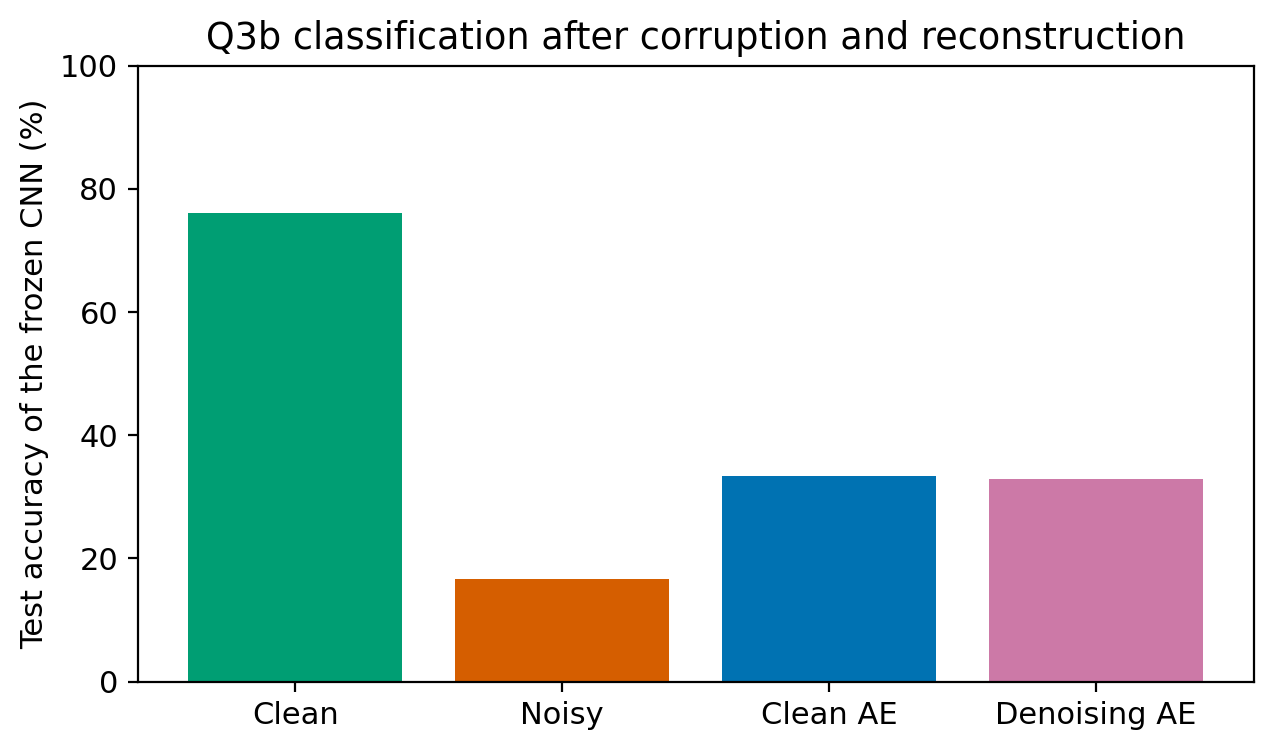
\includegraphics[width=\linewidth]{figures/q3_classify.png}
\caption{Question 3b test accuracy of the frozen CNN.}
\label{fig:q3b}
\end{figure}

\subsection{Class information in the code}
A multinomial logistic regression is fit on the frozen code. Features are standardised with the training-code mean and standard deviation. $C \in \{0.01, 0.1, 1, 10, 100\}$ is chosen by validation accuracy; the smaller $C$ wins a tie. The encoder is not fine-tuned. Some fits hit the 400-iteration limit, so an individual $C$ can be slightly short of its optimum.

Test MSE and test probe accuracy are $0.01160$ and $0.364$ at width 32, $0.00563$ and $0.444$ at 128, and $0.00483$ and $0.545$ at 512 (Figure~\ref{fig:q3c}). Both quantities improve as the code widens. Most of the MSE drop is from 32 to 128. The probe continues to rise from 128 to 512, where the MSE drop is small. The denoiser's code, same width 512, has probe test accuracy $0.539$.

\begin{figure}[t]
\centering
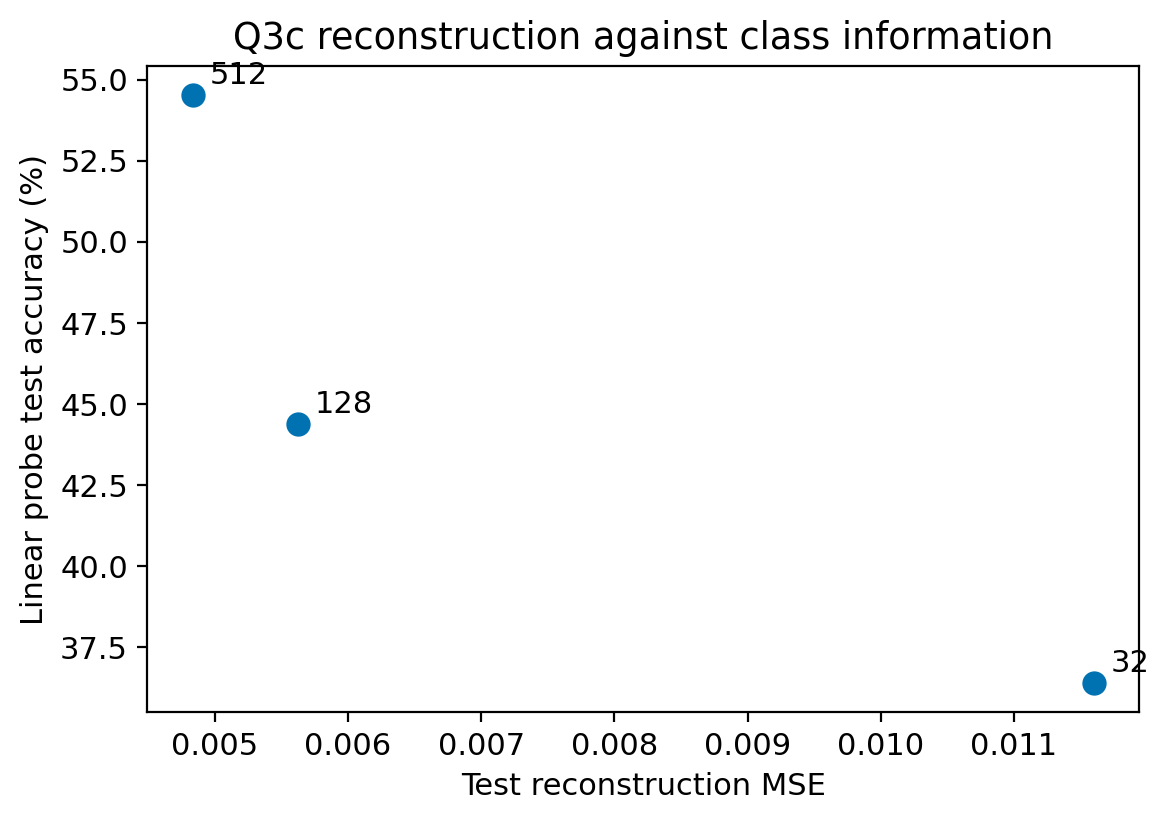
\includegraphics[width=\linewidth]{figures/q3_probe.png}
\caption{Question 3c. Test reconstruction MSE against linear-probe test accuracy. Labels are bottleneck widths.}
\label{fig:q3c}
\end{figure}

\section{Question 4: SVM and clustering}
\subsection{Sweep}
The representation is the 160-dimensional pooled vector of the Question 1a matched CNN, seed 26003, before the linear head. It is frozen. Kernel methods on all 45{,}000 training rows are expensive, so the plan fixes a stratified subset before any fit: 200 images per class, 2{,}000 rows, \texttt{Generator(26003)}, saved in \texttt{splits/q4\_svm\_subset\_seed26003.npy}. Every kernel and every $C$ uses that file. Standardisation is fit on those 2{,}000 rows only.

Kernels are linear, polynomial (degree 3, $\mathrm{coef}_0=1$, $\gamma=\mathrm{scale}$) and RBF ($\gamma=\mathrm{scale}$). Degree and $\gamma$ are not searched. $C \in \{0.01, 0.1, 1, 10, 100\}$ spans four orders of magnitude. The highest validation accuracy wins; a tie keeps the smaller support-vector fraction, then the smaller $C$, then the kernel name alphabetically. Table~\ref{tab:q4} is the full sweep. Figure~\ref{fig:q4} is the selected kernel.

\begin{table}[t]
\centering
\caption{Question 4a. Training accuracy, validation accuracy, and the fraction of the 2{,}000 training rows that are support vectors. The selected row is polynomial, $C{=}1$.}
\label{tab:q4}
\small
\begin{tabular}{llrrr}
\toprule
Kernel & $C$ & Train & Val. & SV \\
\midrule
linear & 0.01 & .910 & .730 & .678 \\
linear & 0.1 & .975 & .719 & .540 \\
linear & 1 & .998 & .709 & .507 \\
linear & 10 & 1.000 & .710 & .503 \\
linear & 100 & 1.000 & .710 & .503 \\
poly & 0.01 & .715 & .640 & .936 \\
poly & 0.1 & .917 & .725 & .761 \\
poly & 1 & .999 & \textbf{.734} & .686 \\
poly & 10 & 1.000 & .726 & .686 \\
poly & 100 & 1.000 & .726 & .686 \\
rbf & 0.01 & .693 & .609 & 1.000 \\
rbf & 0.1 & .754 & .652 & .969 \\
rbf & 1 & .959 & .728 & .814 \\
rbf & 10 & 1.000 & .733 & .810 \\
rbf & 100 & 1.000 & .733 & .810 \\
\bottomrule
\end{tabular}
\end{table}

\begin{figure}[t]
\centering
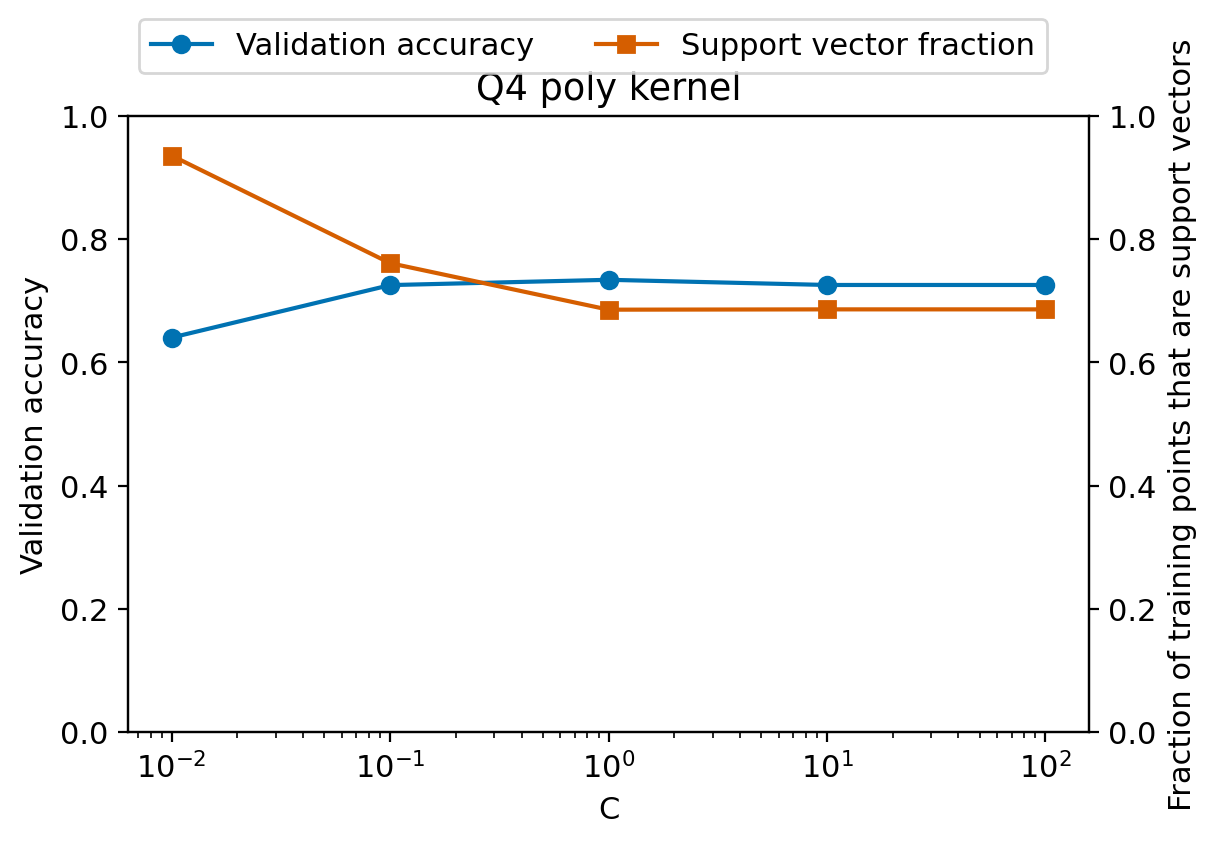
\includegraphics[width=\linewidth]{figures/q4_poly.png}
\caption{Question 4a, polynomial kernel. Validation accuracy and the support-vector fraction against $C$.}
\label{fig:q4}
\end{figure}

Polynomial degree 3 with $C=1$ is the unique validation maximum, at $0.734$, with training accuracy $0.999$ and $68.6\%$ of the rows as support vectors~\cite{cortes1995support}. The single test evaluation is $0.7235$. Small $C$ underfits: RBF at $C=0.01$ has training accuracy $0.693$, validation $0.609$, and every training point is a support vector. Linear overfits as $C$ grows: validation falls from $0.730$ at $C=0.01$ to about $0.710$ once training accuracy has reached 1. Polynomial and RBF are unchanged from $C=10$ to $C=100$.

\subsection{Hard pairs}
After that test evaluation, unordered pairs are ranked by the sum of the two off-diagonal confusion counts. The three largest are cat/dog (358 confusions, $0.179$ of the 2{,}000 images in the pair, 222 support vectors of that binary problem), bird/deer (178, $0.089$, 171 support vectors) and airplane/ship (146, $0.073$, 139 support vectors). The score is the one-versus-one decision column. The cat/dog test image closest to the boundary is an error, with decision score about $0.001$. The pictures are the original RGB images whose features produced those scores; the geometry is in the 160-dimensional code.

\subsection{Clustering}
$k$-means is fit on the same 2{,}000 standardised rows~\cite{macqueen1967kmeans}. Labels are not passed to the fitter. Candidates are $k \in \{5, 8, 10, 12, 15, 20\}$. Validation NMI selects $k$; a tie would keep the $k$ closer to 10, then the smaller $k$. The winning validation NMIs peak at $k=10$ with $0.362$. Test points are assigned by that model. Test labels are used only afterwards. Test ARI is $0.228$~\cite{hubert1985comparing} and test NMI is $0.361$. A majority map from cluster to class, fit on the training subset only, scores $0.460$ on the test set, against the SVM's $0.724$.

The disagreement class under the written rule is bird: SVM recall $0.615$, cluster recall $0.000$, because no training cluster has bird as its majority label (Figure~\ref{fig:q4c}). Automobile is a second large gap ($0.852$ versus $0.417$) but it is not the maximum. The SVM and the clustering do not support the same description of the code.

\begin{figure}[t]
\centering
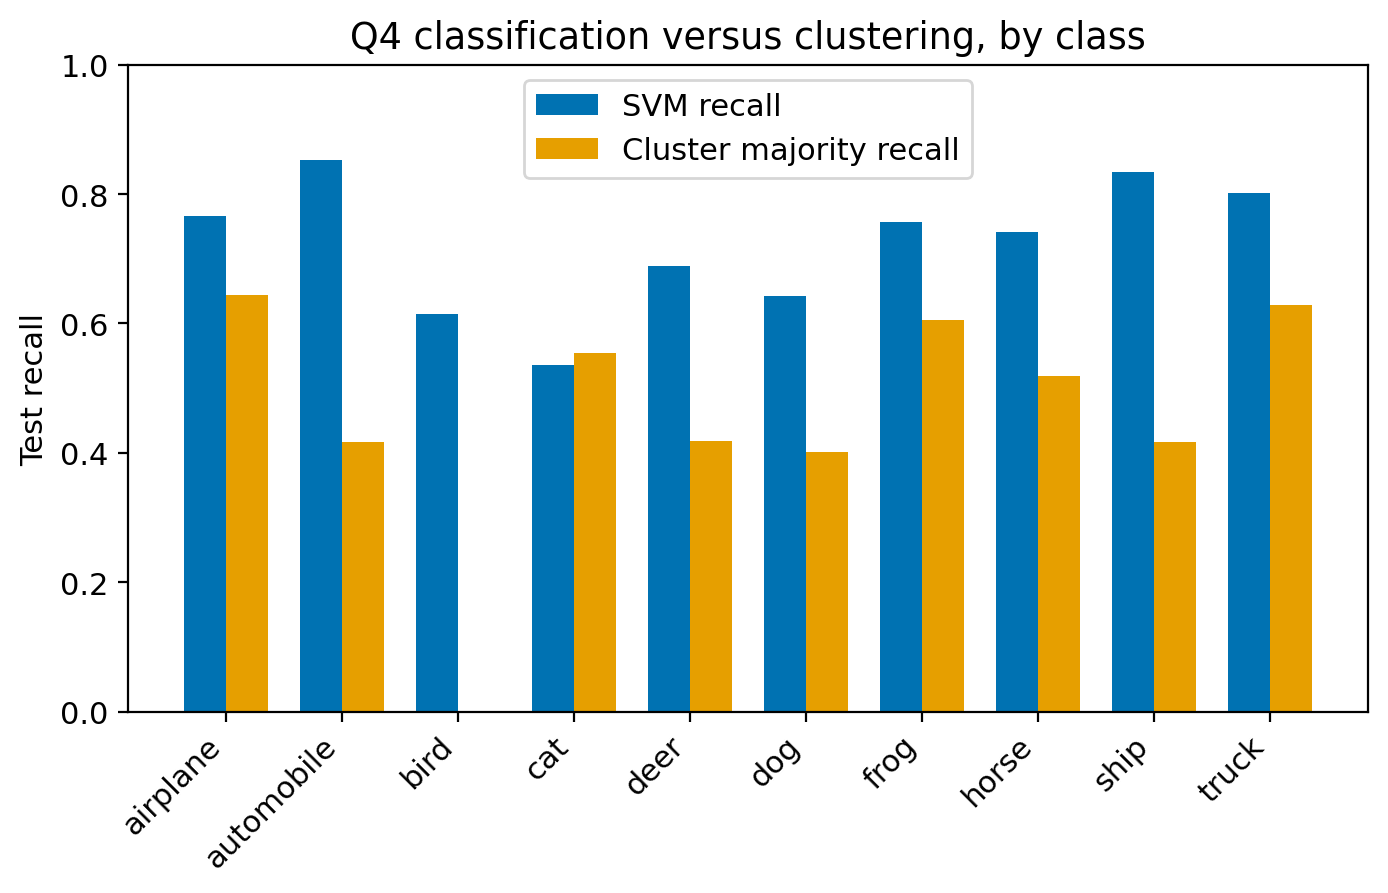
\includegraphics[width=\linewidth]{figures/q4_recall.png}
\caption{Question 4c. Per-class test recall of the selected SVM and of the training-set majority map of $k$-means.}
\label{fig:q4c}
\end{figure}

\section{Discussion and conclusion}
The matched comparison supports missing spatial weight sharing more than capacity or overfitting. The permutation experiment is the clean check: the MLP is unchanged and the CNN falls to the MLP. Grayscale is less stable. Two seeds keep a large CNN lead and one seed does not, so colour is used by both models and is not a sufficient account of the clean-image gap.

Reconstruction quality and linear class information both improve with bottleneck width, but not in proportion. A denoiser that wins on PSNR does not win on the frozen classifier. Pixel fidelity is not the same quantity as the decision the CNN was trained to make.

On one frozen convolutional code, a validation-selected polynomial SVM is accurate and shows the usual small-$C$ underfit and large-$C$ overfit, most clearly for the linear kernel. Clustering the same points without labels recovers a coarser partition and loses bird entirely under a majority map. The two methods disagree, with numbers on both sides.

The main limits are the ones the logs already show. Question 1b did not fit a fully random training set in 40 epochs. One grayscale CNN seed failed. Several logistic probes stopped at 400 iterations. Question 4 uses 2{,}000 stratified rows rather than all 45{,}000, as the kernel budget required; that subset was fixed before selection. There is no git commit yet, so this document has no commit hash.

{\small
\bibliographystyle{ieeenat_fullname}
\bibliography{references}
}

\end{document}
